\documentclass[12pt]{article}
\usepackage{light}

\hidesolutions
%\showsolutions

\begin{document}

\newcommand{\qf}{\text{"}F\text{"}}

\recitation{20}{November 19, 2014}

%%%%%%%%%%%%%%%%%%%%%%%%%%%%%%%%%%%%%%%%%%%%%%%%%%%%%%%%%%%%%%%%%%%%%%%%%%%%%%%

\insolutions{

The Total Probability Law is a handy tool for breaking down the
computation of a probability into distinct cases.

\begin{theorem}[Total Probability Law]
Let $E$ and $X$ be events.  Then
%
\[
\pr{E} = \pr{E \mid X} \cdot \pr{X} +
          \pr{E \mid \overline{X}} \cdot \pr{\overline{X}}
\]
%
provided $0 < \pr{X} < 1$.
\end{theorem}

\begin{proof}
Let's simplify the right side.
%
\begin{align*}
\lefteqn{\pr{E \mid X} \cdot \pr{X} +
	\pr{E \mid \overline{X}} \cdot \pr{\overline{X}}} \hspace{1in} \\
    & = \frac{\pr{E \cap X}}{\pr{X}} \cdot \pr{X} +
	\frac{\pr{E \cap \overline{X}}}{\pr{\overline{X}}} \cdot \pr{\overline{X}} \\
    & = \pr{E \cap X} + \pr{E \cap \overline{X}} \\
    & = \pr{E}
\end{align*}
%
The first step uses the definition of conditional probability.  On the
next-to-last line, we're adding the probabilities of all outcomes in
$E$ \textit{and} $X$ to the probabilities of all outcomes in $E$ and
\textit{not} in $X$.  Since every outcome in $E$ is either in $X$ or
not in $X$, this is the sum of the probabilities of all outcomes in
$E$, which equals $\pr{E}$ by the definition of the probability of an
event.
\end{proof}

The theorem generalizes as follows:
%
\begin{theorem}
Let $E$ be an event and let $X_1, \ldots, X_n$ be disjoint events
whose union is the entire sample space.  Then
%
\[
\pr{E} = \sum_{i=1}^n \pr{E \mid X_i} \cdot \pr{X_i}
\]
%
provided $0 < \pr{X_i} < 1$.
\end{theorem}

%%%%%%%%%%%%%%%%%%%%%%%%%%%%%%%%%%%%%%%%%%%%%%%%%%%%%%%%%%%%%%%%%%%%%%%%%%%%%%%

\newpage
}

\section{Nerditosis}
There is a rare and deadly disease called \textit{Nerditosis} which
afflicts about 1 person in 1000.  One symptom is a compulsion to refer
to everything--- fields of study, classes, buildings, etc.--- using
numbers.  It's horrible.  As victims enter their final, downward
spiral, they're awarded a degree from MIT.  Two doctors claim that
they can diagnose Nerditosis.

\begin{enumerate}
\item Doctor $X$ received his degree from Harvard Medical School.  He
practices at Massachusetts General Hospital and has access to the
latest scanners, lab tests, and research.  Suppose you ask Doctor $X$
whether you have the disease.
%
\begin{itemize}
\item If you have Nerditosis, he says ``yes'' with probability 0.99.
\item If you don't have it, he says ``no'' with probability 0.97.
\end{itemize}
%
Let $D$ be the event that you have the disease, and let $E$ be the
event that the diagnosis is erroneous.  Use the Total Probability Law
to compute $\pr{E}$, the probability that Doctor $X$ makes a mistake.

\solution[\vspace{.9in}]{By the Total Probability Law:
%
\begin{align*}
\pr{E}
    & = \pr{E \mid D} \cdot \pr{D} +
        \pr{E \mid \overline{D}} \cdot \pr{\overline{D}} \\
    & = 0.01 \cdot 0.001 + 0.03 \cdot 0.999 \\
    & = 0.02998
\end{align*}}

\item ``Doctor'' $Y$ received his genuine degree from a
fully-accredited university for \$49.95 via a special internet offer.
He knows that Nerditosis strikes 1 person in 1000, but is a little
shaky on how to interpret this.  So if you ask him whether you have
the disease, he'll helpfully say ``yes'' with probability 1 in 1000
regardless of whether you actually do or not.

Let $D$ be the event that you have the disease, and let $F$ be the
event that the diagnosis is faulty.  Use the Total Probability Law to
compute $\pr{F}$, the probability that Doctor $Y$ made a mistake.

\solution[\vspace{.9in}]{By the Total Probability Law:
%
\begin{align*}
\pr{F}
    & = \pr{F \mid D} \cdot \pr{D} +
        \pr{F \mid \overline{D}} \cdot \pr{\overline{D}} \\
    & = 0.999 \cdot 0.001 + 0.001 \cdot 0.999 \\
    & = 0.001998
\end{align*}}

\item Which doctor is more reliable?

\solution{Doctor $X$ makes more than 15 times as many errors as Doctor
$Y$.}

\end{enumerate}

%%%%%%%%%%%%%%%%%%%%%%%%%%%%%%%%%%%%%%%%%%%%%%%%%%%%%%%%%%%%%%%%%%%%%%%%%%%%%%%

\newpage

\section{Barglesnort}
A Barglesnort makes its lair in one of three caves:
%
\begin{center}
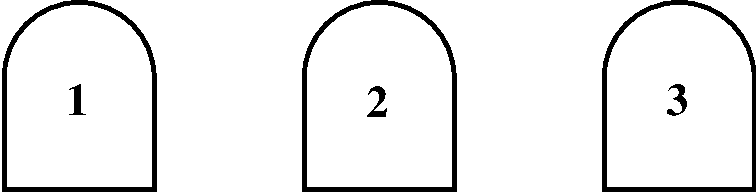
\includegraphics[height=0.75in]{caves}
\end{center}
%
The Barglesnort inhabits cave 1 with probability $\frac{1}{2}$, cave 2
with probability $\frac{1}{4}$, and cave 3 with probability
$\frac{1}{4}$.  A rabbit subsequently moves into one of the two
unoccupied caves, selected with equal probability.  With probability
$\frac{1}{3}$, the rabbit leaves tracks at the entrance to its cave.
(Barglesnorts are much too clever to leave tracks.)  What is the
probability that the Barglesnort lives in cave 3, given that there are
no tracks in front of cave 2?

Use a tree diagram and the four-step method.

\solution{A tree diagram is given below.  Let $B_3$ be the event that
the Barglesnort inhabits cave 3, and let $T_2$ be the event that there
are tracks in front of cave 2.  Taking data from the tree diagram, we
can compute the desired probability as follows:
%
\begin{align*}
\pr{B_3 \mid \overline{T_2}}
	& = \frac{\pr{B_3 \cap \overline{T_2}}}{\pr{\overline{T_2}}} \\
	& = \frac{\frac{1}{24} + \frac{1}{12} + \frac{1}{12}}
		{1 - \frac{1}{12} - \frac{1}{24}} \\
	& = \frac{5}{21}
\end{align*}
%
In the denominator, we apply the formula $\pr{\overline{T_2}} = 1 -
\pr{T_2}$ for convenience.
%
\begin{center}
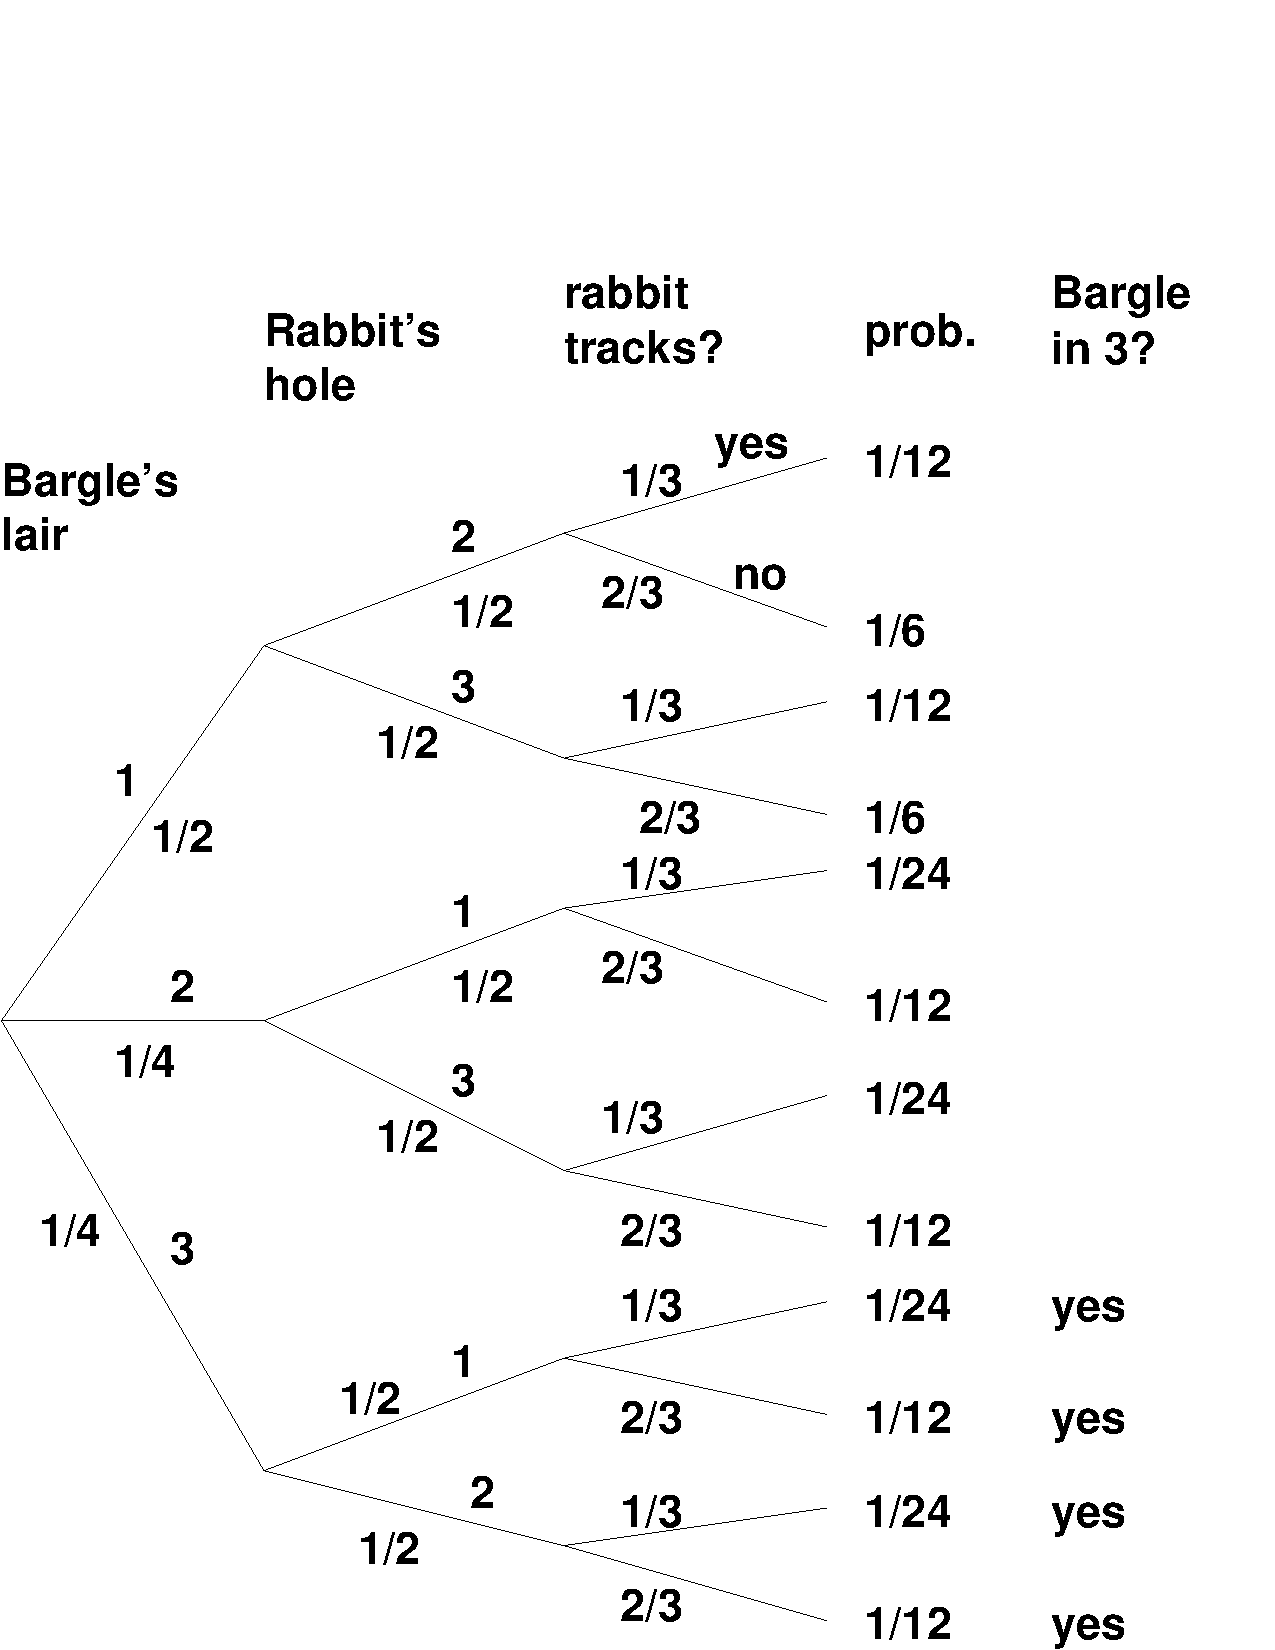
\includegraphics[height=3in]{bargle}
\end{center}
}

%%%%%%%%%%%%%%%%%%%%%%%%%%%%%%%%%%%%%%%%%%%%%%%%%%%%%%%%%%%%%%%%%%%%%%%%%%%%%%%

\newpage

\section{Prisoners}
There are three prisoners in a maximum-security prison for fictional
villains: the Evil Wizard Voldemort, the Dark Lord Sauron, and Little
Bunny Foo-Foo.  The parole board has declared that it will release two
of the three, chosen uniformly at random, but has not yet released
their names.  Naturally, Sauron figures that he will be released to
his home in Mordor, where the shadows lie, with probability
$\frac{2}{3}$.

A guard offers to tell Sauron the name of one of the other prisoners
who will be released (either Voldemort or Foo-Foo).  However, Sauron
declines this offer.  He reasons that if the guard says, for example,
``Little Bunny Foo-Foo will be released'', then his own probability of
release will drop to $\frac{1}{2}$.  This is because he will then know
that either he or Voldemort will also be released, and these two
events are equally likely.

Using a tree diagram and the four-step method, either prove that the
Dark Lord Sauron has reasoned correctly or prove that he is wrong.
Assume that if the guard has a choice of naming either Voldemort or
Foo-Foo (because both are to be released), then he names one of the
two uniformly at random.

\solution{Sauron has reasoned incorrectly.

We can explain the issue in terms of conditional probability.   Let
$S,F,$ and $\qf$ be the events:
\begin{align*}
S & = \text{Sauron is released},\\
F & = \text{Foo-Foo is released},\\
\qf & = \text{Guard says Foo-Foo is released}.
\end{align*}

We can use the tree diagram below to analyze the outcomes and
probabilities we should consider.  The first split in the tree is based on
which two of the three prisoners are to be released, and the second is
based on what the guard tells Sauron.

\bigskip
\centerline{\resizebox{!}{2.8in}{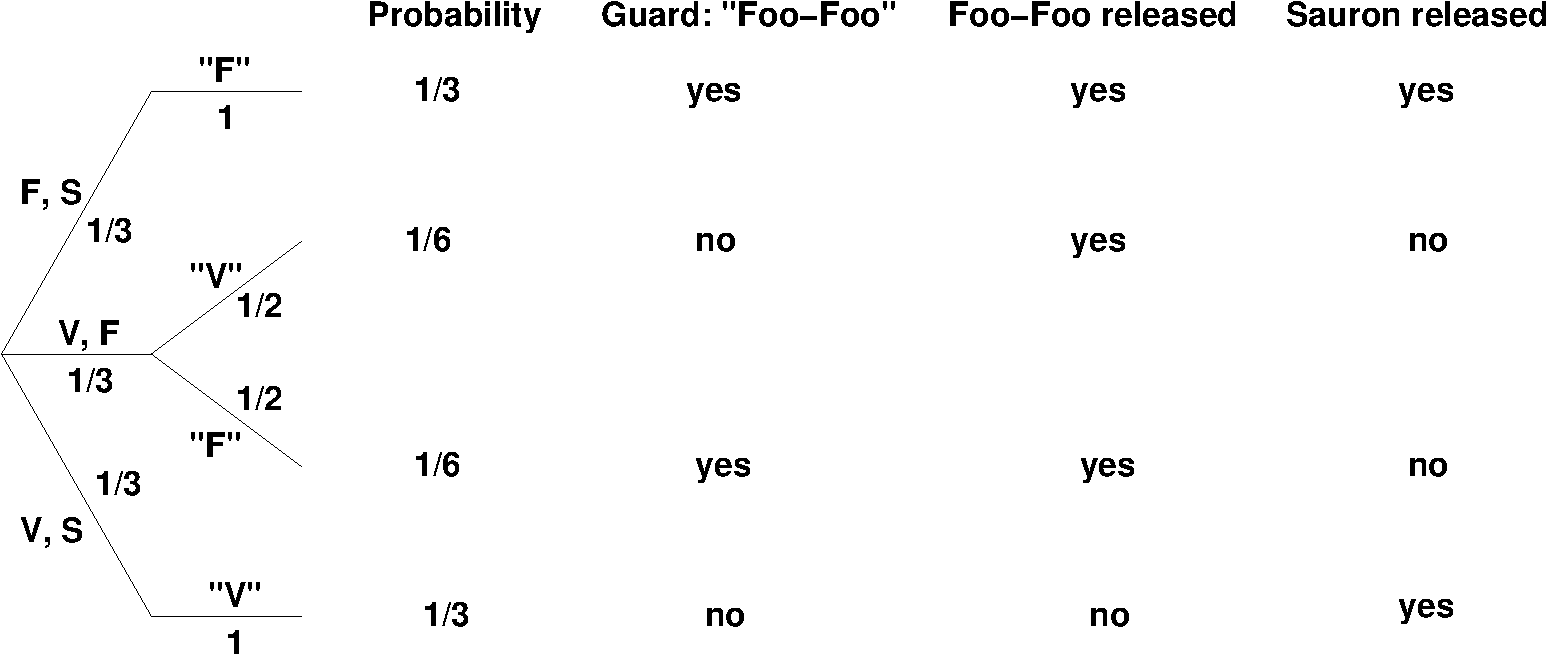
\includegraphics{prison}}}
\bigskip

From the diagram we can see that Sauron has correctly observed that
\[
\pr{S}  = \frac13 + \frac13 = \frac{2}{3}.
\]
And Sauron is correct in reasoning that if event $\qf$ happens, then event
$F$ has also happened.  And he's correct that the probability of his
release given $F$ shrinks to 1/2.  Namely, from the diagram we have:
\begin{align*}
\pr{F} & = \frac13 + \frac16 + \frac16 = \frac23,\\
\pr{S \cap F} & = \frac13\\
\pr{S \mid F} & = \frac{\pr{S \cap F}}{\pr{F}} = \frac{1}{2}.
\end{align*}
So he worries that if he lets $\qf$ happen, then his probability of
release will shrink from 2/3 to $\pr{S \mid F} = 1/2$.

Sauron's confusion is not realizing that the events $F$ and $\qf$ are
different, as the tree makes clear.  These events even have different
probabilities:
\begin{align*}
\pr{\qf} & = \frac13 + \frac16 = \frac{1}{2} \neq \frac23 = \pr{F}.
\end{align*}

Now in determining his probability of release, Sauron should use
\emph{all} the information available.  He should be concerned about his
chances given that \emph{the Guard says} Foo-Foo is released, not merely
given the weaker fact that Foo-Foo is released.  That is, Sauron should
care about $\pr{S \mid \qf}$, not $\pr{S \mid F}$.

We can see from the diagram that
\[
\pr{S \mid \qf}  = \frac{\pr{S \cap \qf}}{\pr{\qf}}
                 = \frac{1/3}{1/2} = \frac{2}{3}
                 = \pr{S}.
\]
So Sauron's probability of release is not changed by hearing from the
guard.}

%%%%%%%%%%%%%%%%%%%%%%%%%%%%%%%%%%%%%%%%%%%%%%%%%%%%%%%%%%%%%%%%%%%%%%%%%%%%%%%

\end{document}

